\documentclass[10pt,article,oneside]{memoir}
\usepackage[top=1.2in, bottom=1.2in, left=1.4in, right=1.4in]{geometry}

\usepackage{amssymb, amsmath, amsthm, mathtools}

% Essential packages
\usepackage{color}
\usepackage{graphicx}
\usepackage{tabularx}
\usepackage{longtable}
\usepackage{enumitem}
\usepackage{url}
\usepackage{float}


% Colors ------------
\usepackage{xcolor}
\definecolor{mygray}{gray}{0.5} % define color on gray scale
\definecolor{lgray}{gray}{0.9} % define color on gray scale
\definecolor{crimson}{RGB}{153,0,0}
\definecolor{dgray}{RGB}{125,125,125}
\newcommand{\crimson}[1]{\textcolor{crimson}{#1}}
  \newcommand{\dgray}[1]{\textcolor{dgray}{#1}}
    \newcommand{\lgray}[1]{\textcolor{lgray}{#1}}
      \newcommand{\mygray}[1]{\textcolor{mygray}{#1}}

% Hyperref
\usepackage[pdfencoding = auto, 
            hidelinks = true, 
            urlcolor = MidnightBlue, 
            linkcolor = MidnighBlue]{hyperref}


% Parameters
\usepackage{soul} % underline
\usepackage{tcolorbox}

% Minion for main text and math
% \usepackage{MinionPro}

% Helvetica for sans serif
% (scaled to match size of Minion)
\usepackage[scaled=0.95]{helvet}

% Bera Mono for monospaced
% (scaled to match size of Minion)
\usepackage[T1]{fontenc}
\usepackage[scaled=0.9]{beramono}
% \usepackage{fontspec}
% \setmonofont[Scale=0.85]{Monaco}

% FORCE HELVET
\renewcommand\familydefault{\sfdefault}

% Spacing
\usepackage{setspace}


% Sectioing
\setcounter{secnumdepth}{0} % fix starting with "0.1"

% Dash 
\renewcommand\labelitemi{--}

% Theorems
\usepackage{etoolbox}
\renewcommand{\qedsymbol}{\rule{0.7em}{0.7em}}
\newtheorem{theorem}{Theorem}
\newtheorem{lem}{Lemma}
\newtheorem{assump}{Assumption}
\theoremstyle{definition}
\newtheorem{definition}{Definition}
\AtEndEnvironment{definition}{\null\hfill\qedsymbol}%
\newtheorem{example}{Example}
\newtheorem{error}{Common Error}
\AtEndEnvironment{error}{\null\hfill\qedsymbol}%

% Math
\newcommand{\var}{\textnormal{Var}}
\newcommand{\cov}{\textnormal{Cov}} 
\newcommand{\cor}{\textnormal{Cor}} 

% Figures
\usepackage{graphicx,grffile}
\makeatletter
\def\maxwidth{\ifdim\Gin@nat@width>\linewidth\linewidth\else\Gin@nat@width\fi}
\def\maxheight{\ifdim\Gin@nat@height>\textheight\textheight\else\Gin@nat@height\fi}
\makeatother

% Scale images if necessary, so that they will not overflow the page
% margins by default, and it is still possible to overwrite the defaults
% using explicit options in \includegraphics[width, height, ...]{}
\setkeys{Gin}{width=\maxwidth,height=\maxheight,keepaspectratio}


% Shading and Rmd macros
\usepackage{color}
\usepackage{fancyvrb}
\newcommand{\VerbBar}{|}
\newcommand{\VERB}{\Verb[commandchars=\\\{\}]}
\DefineVerbatimEnvironment{Highlighting}{Verbatim}{commandchars=\\\{\}}
% Add ',fontsize=\small' for more characters per line
\usepackage{framed}
\definecolor{shadecolor}{RGB}{248,248,248}
\newenvironment{Shaded}{\begin{snugshade}}{\end{snugshade}}
\newcommand{\AlertTok}[1]{\textcolor[rgb]{0.94,0.16,0.16}{#1}}
\newcommand{\AnnotationTok}[1]{\textcolor[rgb]{0.56,0.35,0.01}{\textbf{\textit{#1}}}}
\newcommand{\AttributeTok}[1]{\textcolor[rgb]{0.77,0.63,0.00}{#1}}
\newcommand{\BaseNTok}[1]{\textcolor[rgb]{0.00,0.00,0.81}{#1}}
\newcommand{\BuiltInTok}[1]{#1}
\newcommand{\CharTok}[1]{\textcolor[rgb]{0.31,0.60,0.02}{#1}}
\newcommand{\CommentTok}[1]{\textcolor[rgb]{0.56,0.35,0.01}{\textit{#1}}}
\newcommand{\CommentVarTok}[1]{\textcolor[rgb]{0.56,0.35,0.01}{\textbf{\textit{#1}}}}
\newcommand{\ConstantTok}[1]{\textcolor[rgb]{0.00,0.00,0.00}{#1}}
\newcommand{\ControlFlowTok}[1]{\textcolor[rgb]{0.13,0.29,0.53}{\textbf{#1}}}
\newcommand{\DataTypeTok}[1]{\textcolor[rgb]{0.13,0.29,0.53}{#1}}
\newcommand{\DecValTok}[1]{\textcolor[rgb]{0.00,0.00,0.81}{#1}}
\newcommand{\DocumentationTok}[1]{\textcolor[rgb]{0.56,0.35,0.01}{\textbf{\textit{#1}}}}
\newcommand{\ErrorTok}[1]{\textcolor[rgb]{0.64,0.00,0.00}{\textbf{#1}}}
\newcommand{\ExtensionTok}[1]{#1}
\newcommand{\FloatTok}[1]{\textcolor[rgb]{0.00,0.00,0.81}{#1}}
\newcommand{\FunctionTok}[1]{\textcolor[rgb]{0.00,0.00,0.00}{#1}}
\newcommand{\ImportTok}[1]{#1}
\newcommand{\InformationTok}[1]{\textcolor[rgb]{0.56,0.35,0.01}{\textbf{\textit{#1}}}}
\newcommand{\KeywordTok}[1]{\textcolor[rgb]{0.13,0.29,0.53}{\textbf{#1}}}
\newcommand{\NormalTok}[1]{#1}
\newcommand{\OperatorTok}[1]{\textcolor[rgb]{0.81,0.36,0.00}{\textbf{#1}}}
\newcommand{\OtherTok}[1]{\textcolor[rgb]{0.56,0.35,0.01}{#1}}
\newcommand{\PreprocessorTok}[1]{\textcolor[rgb]{0.56,0.35,0.01}{\textit{#1}}}
\newcommand{\RegionMarkerTok}[1]{#1}
\newcommand{\SpecialCharTok}[1]{\textcolor[rgb]{0.00,0.00,0.00}{#1}}
\newcommand{\SpecialStringTok}[1]{\textcolor[rgb]{0.31,0.60,0.02}{#1}}
\newcommand{\StringTok}[1]{\textcolor[rgb]{0.31,0.60,0.02}{#1}}
\newcommand{\VariableTok}[1]{\textcolor[rgb]{0.00,0.00,0.00}{#1}}
\newcommand{\VerbatimStringTok}[1]{\textcolor[rgb]{0.31,0.60,0.02}{#1}}
\newcommand{\WarningTok}[1]{\textcolor[rgb]{0.56,0.35,0.01}{\textbf{\textit{#1}}}}


% Parmaters

\title{ \LARGE\textbf{CCES Cumulative Common Content (2006 - 2018)}}

\author{Shiro Kuriwaki\thanks{Department of Government, Harvard University. ORCID:
\url{https://orcid.org/0000-0002-5687-2647}. Bug reports welcome. My
thanks to Alexander Agadjanian, Steve Ansolabehere, Stephen DiMauro,
Bernard Fraga, Nathan Kaplan, Mayya Komisarchik, and Stephen Pettigrew
for their contributions. Thanks to Joe Williams at YouGov, and Jon
Keane, Mike Malecki, and Gordon Shotwell atCrunch for their help.}  }


\date{Guide last updated: 2019-09-05}

\begin{document}

\maketitle





\renewcommand\UrlFont{\color{crimson}\ttfamily}

\emph{To cite the dataset:}

\begin{quote}
Kuriwaki, Shiro, 2018, ``Cumulative CCES Common Content (2006-2018)'',
\href{https://dataverse.harvard.edu/dataset.xhtml?persistentId=doi:10.7910/DVN/II2DB6}{\url{doi:10.7910/DVN/II2DB6}},
Harvard Dataverse
\end{quote}

This dataset combines thirteen years (2006 - 2018) of the Cooperative
Congressional Election Study (Principal Investigators: Stephen
Ansolabehere, Sam Luks, Brian Schaffner).

\smallskip

The Cooperative Congressional Election Study (CCES) is an online survey
conducted around November of each year, asking a range of questions on
political behavior and public opinion. Questions can change from year to
year; this cumulative file includes only standard questions asked
multiple years.

\smallskip

This dataset was constructed from CCES datasets from each year. The
final product is a \texttt{tibble}-style data frame (built in R) that is
also available as a Stata \texttt{dta} file. In addition, the same
dataset is available on \texttt{Crunch}, an analytics interface
optimized for survey datasets.

\smallskip

Please note that this cumulative dataset makes some modifications to the
original CCES datasets for comparability. These modifications are only
made when differences are deemed sufficiently minor, and are documented
in source code (see below). However, for details on the survey
methodology and a list of all questions, readers should consult the
guides for each year.

\vspace{1cm}

\noindent\makebox[\textwidth][c]{%
\begin{minipage}{0.92\linewidth}
\begin{itemize}\addtolength{\itemsep}{10pt}

\item \textbf{To see the source code, } report a bug, or ask a question about the data, please feel free to file an issue from the source code page:  \url{https://github.com/kuriwaki/cces_cumulative}. Alternatively, please contact me by email.

\item \textbf{To obtain the individual year's CCES datasets, } search the CCES dataverse (\url{https://dataverse.harvard.edu/dataverse/cces}) or access the CCES homepage (\url{https://cces.gov.harvard.edu/}). Sign-up to the Crunch dataset from the homepage as well.

\item \textbf{To examine the survey methodology, } consult the Frequently Asked Questions page (\url{https://cces.gov.harvard.edu/frequently-asked-questions}) or the  Methodology section of a recent Common Content's codebook (\url{https://doi.org/10.7910/DVN/GDF6Z0}).
\end{itemize}
\end{minipage}
}

\newpage
\setcounter{tocdepth}{3}
\tableofcontents*

\newpage

\hypertarget{getting-started}{%
\section{Getting Started}\label{getting-started}}

The \texttt{.Rds} format can be read into R. This format preserves
dataset properties such as the distinction between integers and doubles,
and labelled variables. Unlike a \texttt{.Rdata} file, an \texttt{.Rds}
file is assigned to an object.

\begin{Shaded}
\begin{Highlighting}[]
\NormalTok{cc <-}\StringTok{ }\KeywordTok{readRDS}\NormalTok{(}\StringTok{"cumulative_2006_2018.Rds"}\NormalTok{)}
\end{Highlighting}
\end{Shaded}

The dataset in R is best viewed in \texttt{dplyr}, although it can also
be analyzed as a standard data frame.

\begin{Shaded}
\begin{Highlighting}[]
\KeywordTok{library}\NormalTok{(tidyverse)}
\NormalTok{cc}
\end{Highlighting}
\end{Shaded}

A Stata dta file is provided as well.
\texttt{cumulative\_2006\_2018.dta} can be read by Stata, or in R by the
\texttt{haven} package

\begin{Shaded}
\begin{Highlighting}[]
\KeywordTok{library}\NormalTok{(haven)}
\NormalTok{cc <-}\StringTok{ }\KeywordTok{read_dta}\NormalTok{(}\StringTok{"cumulative_2006_2018.dta"}\NormalTok{)}
\end{Highlighting}
\end{Shaded}

\hypertarget{labelled-variables-for-analysis-in-r}{%
\subsection{Labelled variables (for analysis in
R)}\label{labelled-variables-for-analysis-in-r}}

A note on variable types. The R dataset stores variables in
\texttt{numeric}, \texttt{character}, \texttt{factor}, or
\texttt{labelled} class.\footnote{Technically, this is now called a
  \texttt{labelled\_haven} class, to disambiguate from an unrelated but
  older use of \texttt{labelled} in the Hmisc package.} The first three
classes are commonly used, but the \texttt{lablelled} format is more
novel. \texttt{labelled} classes are numeric integers where each integer
is associated with a label (See vignette
\href{https://cran.r-project.org/web/packages/labelled/vignettes/intro_labelled.html}{here}).
This makes it the same as \texttt{factor} but alwasys ordered and
referenceable by its numeric value. It is essentially the same idea as
labels in Stata and SPSS. It is built around R's \texttt{haven} package,
which includes more documentation.

A labelled variable's labels are not usually shown. Recent versions of
the \texttt{haven} package (version 2.1.0 or above) will display the
associated labels in the Console if selected within a tibble (a
dataframe in tidyverse). This makes it immediately obvious which value
is associated with which label.

\begin{Shaded}
\begin{Highlighting}[]
\KeywordTok{select}\NormalTok{(cc, year, case_id, pid3)}
\end{Highlighting}
\end{Shaded}

\begin{verbatim}
# A tibble: 452,755 x 3
    year case_id            pid3
   <int>   <int>       <int+lbl>
 1  2006  439219 1 [Democrat]   
 2  2006  439224 4 [Other]      
 3  2006  439228 1 [Democrat]   
 4  2006  439237 1 [Democrat]   
 5  2006  439238 1 [Democrat]   
 6  2006  439242 3 [Independent]
 7  2006  439251 2 [Republican] 
 8  2006  439254 1 [Democrat]   
 9  2006  439255 1 [Democrat]   
10  2006  439263 1 [Democrat]   
# ... with 452,745 more rows
\end{verbatim}

But labels can be made explicit transforming the labelled vector into a
factor. On the other hand, removes the numerical ordering and value
codes in the labelled class.

\begin{Shaded}
\begin{Highlighting}[]
\KeywordTok{library}\NormalTok{(haven)}
\KeywordTok{select}\NormalTok{(cc, year, case_id, pid3) }\OperatorTok\StringTok{ }
\StringTok{  }\KeywordTok{mutate}\NormalTok{(}\DataTypeTok{pid3_fct =} \KeywordTok{as_factor}\NormalTok{(pid3))}
\end{Highlighting}
\end{Shaded}

\begin{verbatim}
# A tibble: 452,755 x 4
    year case_id            pid3 pid3_fct   
   <int>   <int>       <int+lbl> <fct>      
 1  2006  439219 1 [Democrat]    Democrat   
 2  2006  439224 4 [Other]       Other      
 3  2006  439228 1 [Democrat]    Democrat   
 4  2006  439237 1 [Democrat]    Democrat   
 5  2006  439238 1 [Democrat]    Democrat   
 6  2006  439242 3 [Independent] Independent
 7  2006  439251 2 [Republican]  Republican 
 8  2006  439254 1 [Democrat]    Democrat   
 9  2006  439255 1 [Democrat]    Democrat   
10  2006  439263 1 [Democrat]    Democrat   
# ... with 452,745 more rows
\end{verbatim}

and unlike factors, they can be referenced by their underlying numeric
value. In short, it is sometimes useful to treat survey values as
numbers rather than raw text, and the labelled calss allows you to do
that.

\begin{Shaded}
\begin{Highlighting}[]
\KeywordTok{select}\NormalTok{(cc, year, case_id, pid3) }\OperatorTok\StringTok{ }
\StringTok{  }\KeywordTok{filter}\NormalTok{(pid3 }\OperatorTok{==}\StringTok{ }\DecValTok{1}\NormalTok{)}
\end{Highlighting}
\end{Shaded}

\begin{verbatim}
# A tibble: 160,637 x 3
    year case_id         pid3
   <int>   <int>    <int+lbl>
 1  2006  439219 1 [Democrat]
 2  2006  439228 1 [Democrat]
 3  2006  439237 1 [Democrat]
 4  2006  439238 1 [Democrat]
 5  2006  439254 1 [Democrat]
 6  2006  439255 1 [Democrat]
 7  2006  439263 1 [Democrat]
 8  2006  439304 1 [Democrat]
 9  2006  439338 1 [Democrat]
10  2006  439390 1 [Democrat]
# ... with 160,627 more rows
\end{verbatim}

Some variables are stored as labelled values, and some are not and
stored as factors. Most of this is because the latter variables were
different enough in their value codings across years that summarizing
them into a single numeric value was difficult.

\hypertarget{adding-more-variables}{%
\subsection{Adding more variables}\label{adding-more-variables}}

As noted, the cumulative dataset only uses key variables from each
year's common content. However,common content variables can be merged
in.

In R, one could use the \texttt{merge} or \texttt{left\_join} functions.
Here is sample code for merging with the latter. In Stata, users can use
\texttt{merge\ 1:1}. In all cases, \texttt{year} and \texttt{case\_id}
uniquely identify every row in the common content, so merges should
merge on year and the case identifier.

\newpage

\hypertarget{features-of-the-2006---2018-cumulative-dataset}{%
\section{Features of the 2006 - 2018 Cumulative
Dataset}\label{features-of-the-2006---2018-cumulative-dataset}}

\hypertarget{unified-variable-names}{%
\subsection{Unified Variable Names}\label{unified-variable-names}}

Most variables in this dataset come straight from each year's CCES.
However, it renames and standardizes variable names, making them
accessible in one place. Please see the rest of this guide or the Crunch
dataset for a full list and description of variables.

\hypertarget{chosen-candidate-names-and-identifiers}{%
\subsection{Chosen Candidate Names and
Identifiers}\label{chosen-candidate-names-and-identifiers}}

One addition to this cumulative dataset are variables of candidate names
and identifiers that a respondent chose. In the individual year's CCES
datasets, typically the response values for a vote choice question is a
generic label, e.g. \texttt{Candidate1} and \texttt{Candidate2}. Then,
separate variables of names and parties correspond to each
\texttt{Candidate1} and \texttt{Candidate2}.

Instead, the cumulative dataset shows both the generic label \emph{and}
the chosen candidate's name and party, which will vary across
individuals.

\begin{Shaded}
\begin{Highlighting}[]
\KeywordTok{select}\NormalTok{(cc, year, case_id, st, }\KeywordTok{matches}\NormalTok{(}\StringTok{"voted_sen"}\NormalTok{))}
\end{Highlighting}
\end{Shaded}

\begin{verbatim}
# A tibble: 452,755 x 7
    year case_id st    voted_sen voted_sen_party voted_sen_chosen
   <int>   <int> <chr> <fct>     <fct>           <chr>           
 1  2006  439219 NC    <NA>      <NA>            <NA>            
 2  2006  439224 OH    [Democra~ Democratic      Sherrod C. Brow~
 3  2006  439228 NJ    [Democra~ Democratic      Robert Menendez~
 4  2006  439237 IL    <NA>      <NA>            <NA>            
 5  2006  439238 NY    [Democra~ Democratic      Hillary Rodham ~
 6  2006  439242 TX    I Did No~ <NA>            <NA>            
 7  2006  439251 MN    [Republi~ Republican      Mark Kennedy (R)
 8  2006  439254 NV    [Democra~ Democratic      Jack Carter (D) 
 9  2006  439255 TX    [Democra~ Democratic      Barbara Ann Rad~
10  2006  439263 MD    I Did No~ <NA>            <NA>            
# ... with 452,745 more rows, and 1 more variable: voted_sen_fec <chr>
\end{verbatim}

\hypertarget{crunch}{%
\subsection{Crunch}\label{crunch}}

A version of the dataset is also included in Crunch, a database platform
that makes it easy to view and analyze survey data either with our
without any programming experience.

\begin{enumerate}
\def\labelenumi{\arabic{enumi}.}
\tightlist
\item
  Obtain Access: For View access to the dataset (free), please sign up
  here:
  \url{https://harvard.az1.qualtrics.com/jfe/form/SV_066hQi4Eeco3Kap}.
  For questions and more access, please contact the CCES Team.
\end{enumerate}

\newpage

\begin{enumerate}
\def\labelenumi{\arabic{enumi}.}
\setcounter{enumi}{1}
\tightlist
\item
  Browse: Crunch offers a web GUI for quickly browsing variables:
\end{enumerate}

\begin{figure}[H]
\centering
\centerline{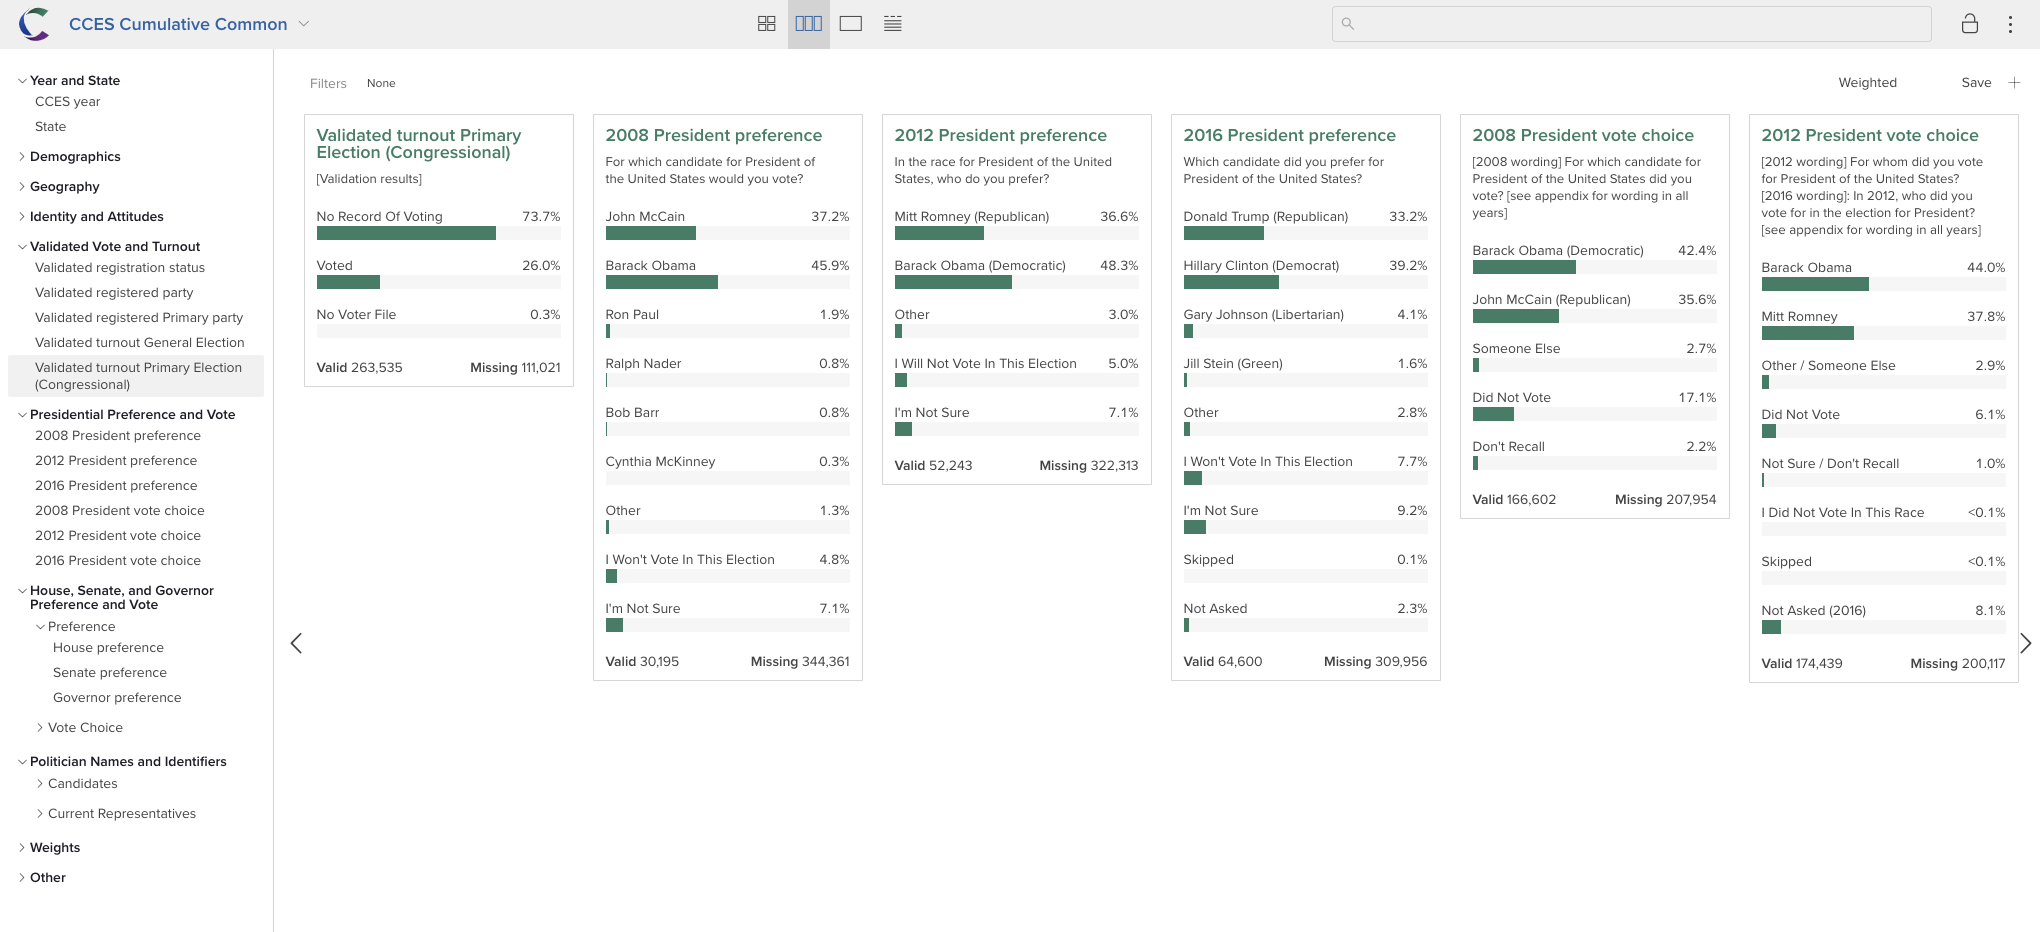
\includegraphics[width=1.05\linewidth]{01_crunch_browse.png}}
\end{figure}

\begin{enumerate}
\def\labelenumi{\arabic{enumi}.}
\setcounter{enumi}{2}
\tightlist
\item
  Analyze: The crunch interface allows Viewers to make cross-tabs and
  bar graphs quickly.\\

  \begin{figure}[H]
  \centering
  \centerline{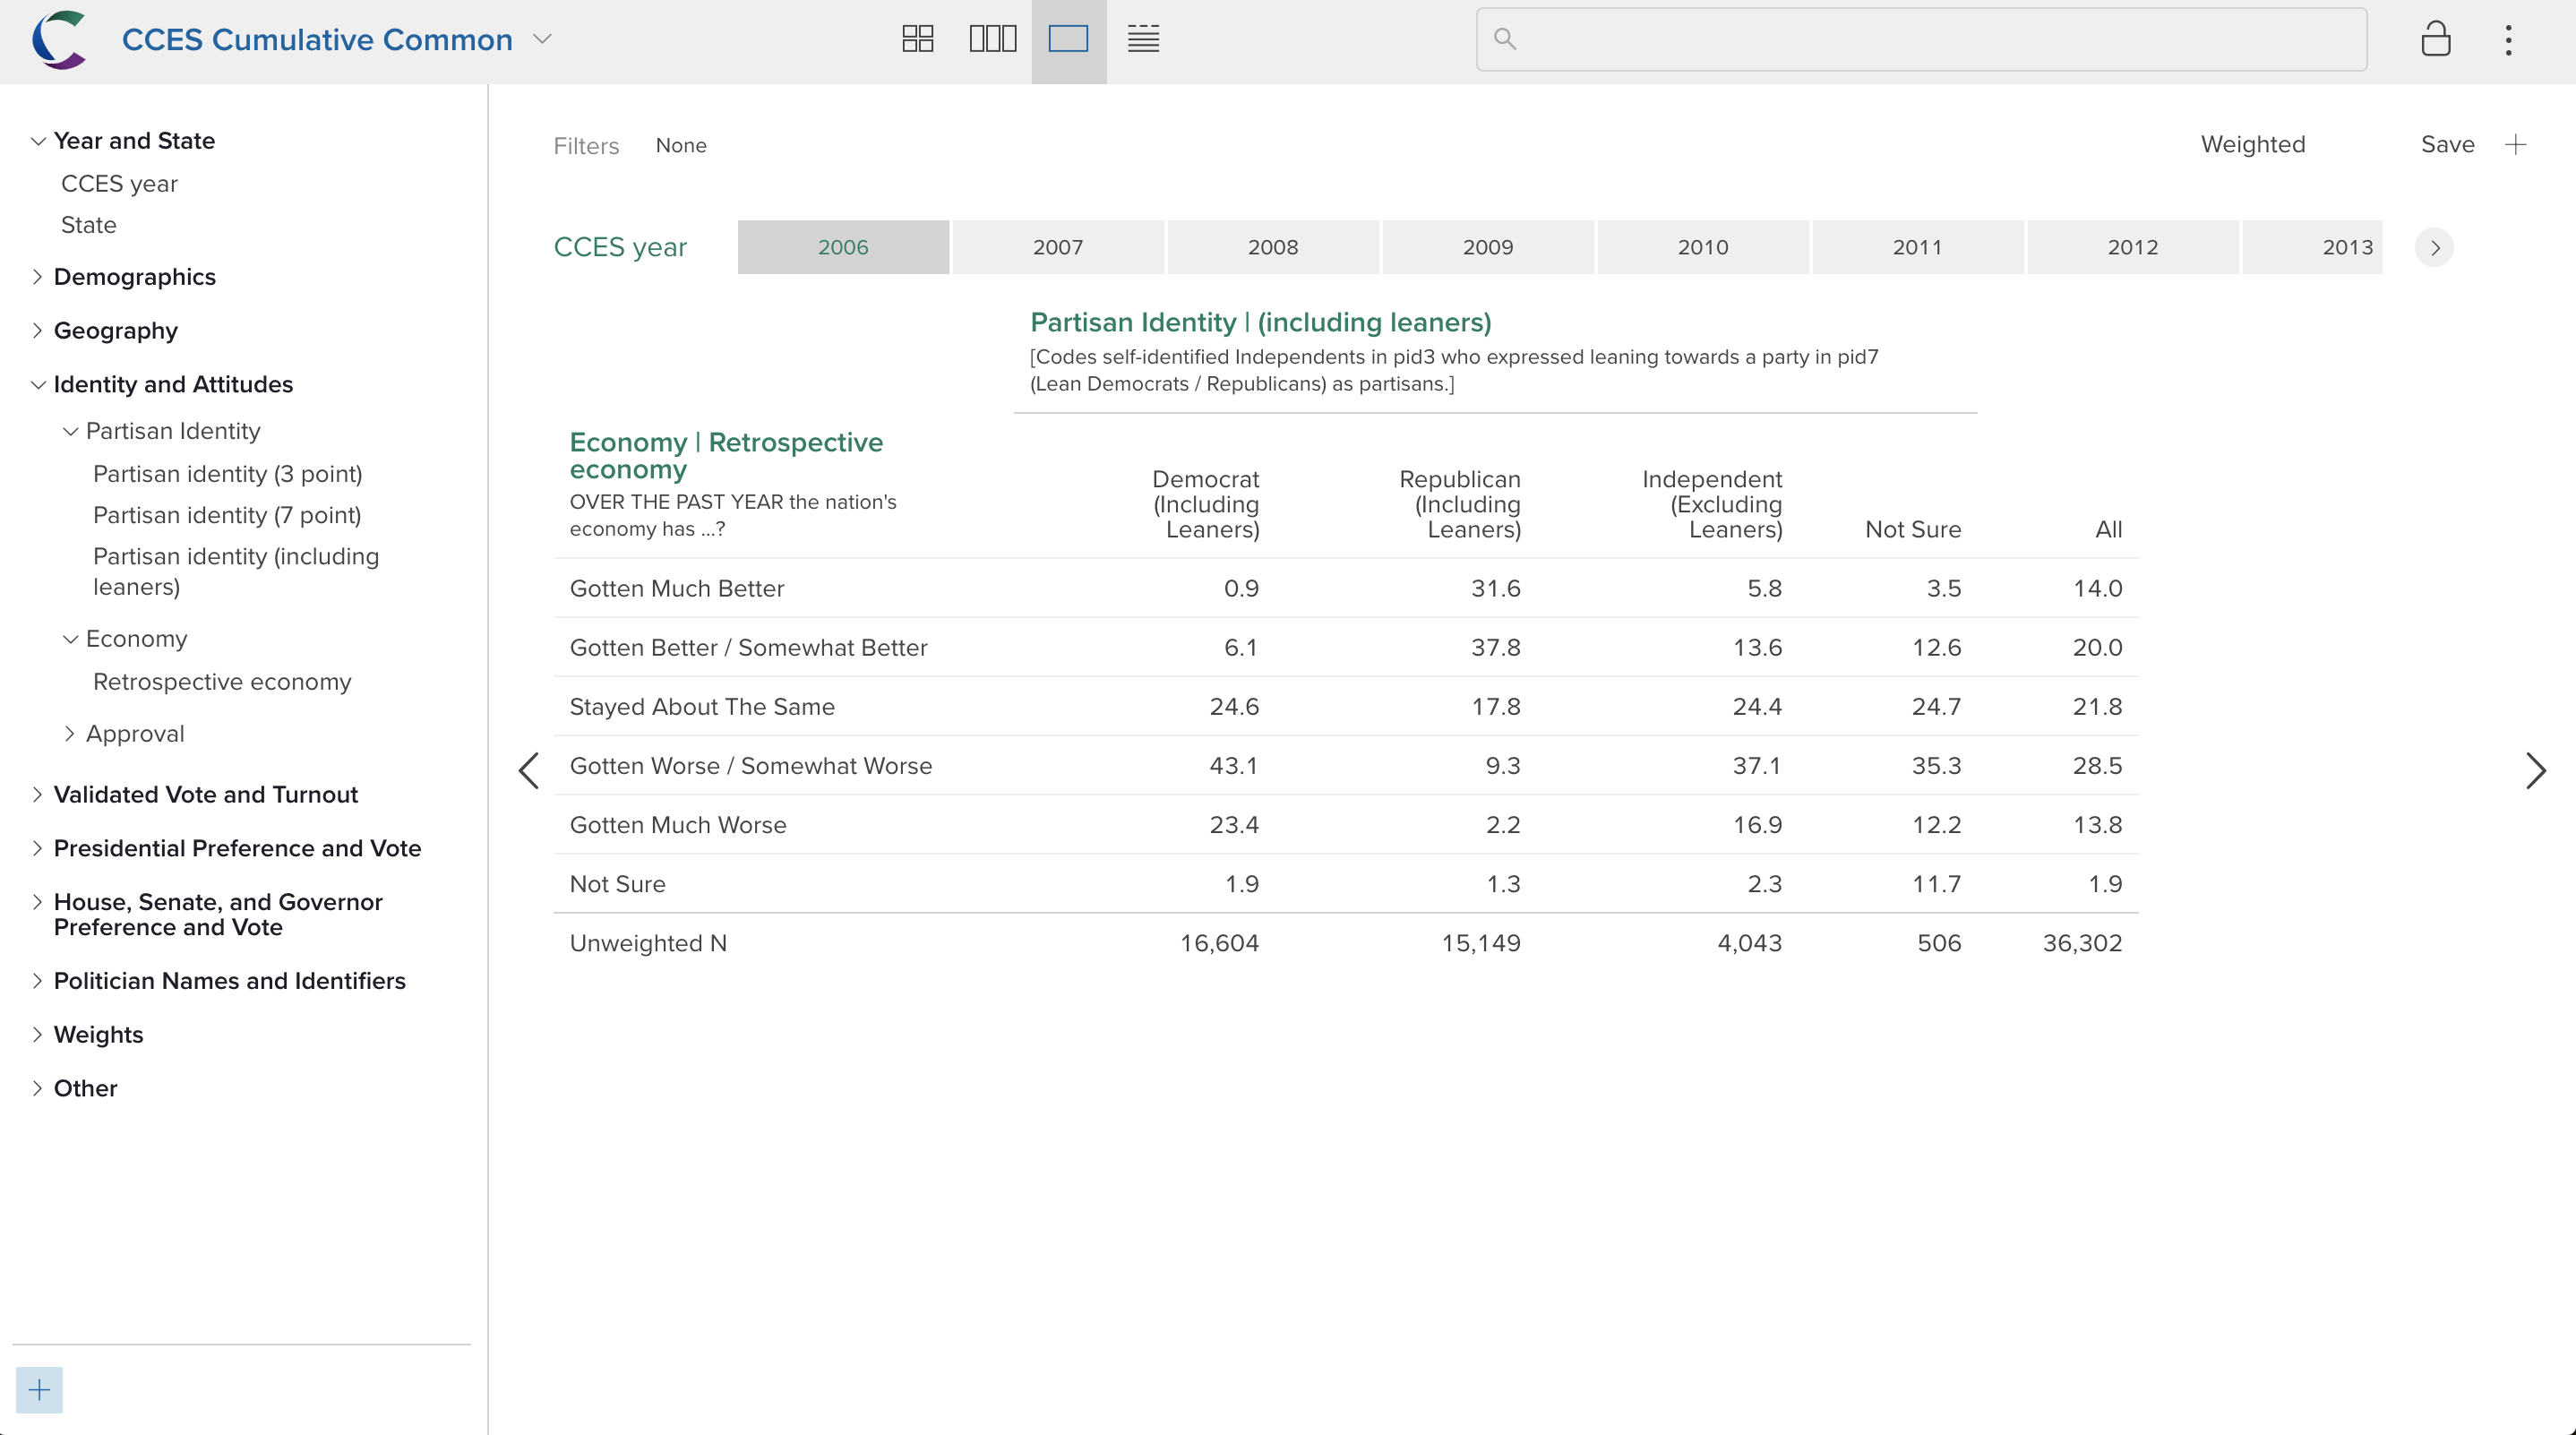
\includegraphics[width=1.05\linewidth]{02_crunch_tab.png}}
  \end{figure}
\end{enumerate}

Crunch datasets can also be manipulated from a R package,
\texttt{crunch} \url{https://github.com/Crunch-io/rcrunch}. To learn
more about the features, please take a look at their homepage
\textless{}crunch.io\textgreater{} or their
\href{https://www.youtube.com/watch?v=zA7N_Q1EpSs}{5-minute demo video}.

\newpage

\hypertarget{variables}{%
\section{Variables}\label{variables}}

The sections below provide summary more information on each variable.

\begin{itemize}
\tightlist
\item
  The title shows the name of the variable as it appears in the dataset
  (``alias'' in Crunch terminology), followed by a more descriptive name
  suitable for presentation (``name'' in Crunch terminology).
\item
  Question wordings, where applicable, immediately follow. Otherwise a
  description is provided in square brackets (\texttt{{[}\ \ {]}}). All
  square brackets, both in the description and the response options,
  indicate descriptions that are summaries rather than the question
  verbatim.
\item
  A tabulation of response options (or summary statistics for numeric
  variables) follow. Numbers are unweighted counts.
\item
  The ``Years'' bullet lists the years of the CCES in which data on the
  variable is available at all. If a year is not listed, either the
  question was not asked in the year or was not incorporated in the
  creation of this dataset.
\item
  Finally, the ``Limitations'' bullet notes some of the caveats required
  when interpreting this variable. As this dataset is combinations of
  different surveys, some year-specific details on implementation are
  inevitably lost. For example, for all 2016 responses ``Not Asked'' and
  ``Skipped'' are both coded as a \texttt{NA} (missing) to stay
  consistent with past years that did not make that finer distinction.
\end{itemize}

\hypertarget{administration}{%
\section{Administration}\label{administration}}

\hypertarget{year-cces-year}{%
\subsubsection{\texorpdfstring{\texttt{year}: CCES
year}{year: CCES year}}\label{year-cces-year}}

{[}Year of CCES Common Content{]}

\begin{table}[H]
\centering
\begin{tabular}{lr}
\toprule
 & n\\
\midrule
2006 & 36,421\\
2007 & 9,999\\
2008 & 32,800\\
2009 & 13,800\\
2010 & 55,400\\
2011 & 20,150\\
2012 & 54,535\\
2013 & 16,400\\
2014 & 56,200\\
2015 & 14,250\\
2016 & 64,600\\
2017 & 18,200\\
2018 & 60,000\\
\bottomrule
\end{tabular}
\end{table}

\hypertarget{starttime-start-time}{%
\subsubsection{\texorpdfstring{\texttt{starttime}: Start
time}{starttime: Start time}}\label{starttime-start-time}}

{[}Pre-election wave start time (up to second){]}

\begin{verbatim}
                 Min.               1st Qu.                Median 
"2006-10-07 00:02:34" "2012-10-12 14:48:08" "2014-10-20 15:49:08" 
                 Mean               3rd Qu.                  Max. 
"2014-08-30 23:43:39" "2016-10-21 08:26:27" "2018-11-05 23:27:49" 
                 NA's 
             "118349" 
\end{verbatim}

\begin{itemize}
\tightlist
\item
  Years: 2006, 2009, 2012, 2013, 2014, 2015, 2016, 2017, 2018
\end{itemize}

\hypertarget{tookpost-took-post-election-wave}{%
\subsubsection{\texorpdfstring{\texttt{tookpost}: Took post-election
wave}{tookpost: Took post-election wave}}\label{tookpost-took-post-election-wave}}

{[}Whether or not the respondent took the post-election wave of the
survey (in even years){]}

\begin{table}[H]
\centering
\begin{tabular}{lr}
\toprule
 & n\\
\midrule
Did Not Take Post-Election Survey & 59,064\\
Took Post-Election Survey & 300,892\\
(Missing) & 92,799\\
\bottomrule
\end{tabular}
\end{table}

\begin{itemize}
\tightlist
\item
  Years: 2006, 2008, 2010, 2012, 2014, 2016, 2018 (Post-election wave
  only exists for even years)
\end{itemize}

\hypertarget{weights}{%
\section{Weights}\label{weights}}

\hypertarget{weight-survey-weight-year-specific}{%
\subsubsection{\texorpdfstring{\texttt{weight}: Survey weight
(Year-Specific)}{weight: Survey weight (Year-Specific)}}\label{weight-survey-weight-year-specific}}

{[}weights for pre-election survey of each year{]}

\begin{verbatim}
   Min. 1st Qu.  Median    Mean 3rd Qu.    Max. 
 0.0000  0.4259  0.7281  1.0000  1.1741 15.0006 
\end{verbatim}

\begin{itemize}
\tightlist
\item
  Years: All of 2006-2018
\item
  In even years, they are re-computed after vote validation has been
  computed and those re-computed weights are taken here when available.
  The weights applied to the sample (which is originally drawn from a
  matched sample) are constructed to make each year's respondents' pool
  representative of the national adult population. See the methodology
  section of the
  \href{https://dataverse.harvard.edu/api/access/datafile/3047286}{2016
  Guide} for details.
\item
  Limitations: Only specific to each year. Built off of the entire
  pre-election wave sample, but not necessarily to adjust post-election
  wave respondents. See \texttt{weight\_post}
\end{itemize}

\hypertarget{weight_cumulative-survey-weight-cumulative}{%
\subsubsection{\texorpdfstring{\texttt{weight\_cumulative}: Survey
weight
(Cumulative)}{weight\_cumulative: Survey weight (Cumulative)}}\label{weight_cumulative-survey-weight-cumulative}}

{[}weight variable with simple adjustment: multiplied a constant within
year to make years comparable{]}

\begin{verbatim}
   Min. 1st Qu.  Median    Mean 3rd Qu.    Max. 
 0.0000  0.2989  0.5562  0.9418  1.0754 24.0297 
\end{verbatim}

\begin{itemize}
\tightlist
\item
  Years: All of 2006-2018
\item
  Limitations: Only a simple transformation of \texttt{weight}.
  Specifically, \texttt{weight\_cumulative} is \texttt{weight} divided
  by the year-specific factors shown in the following table. For
  example, all weights in the 2016 common content are divided by about
  1.97, because it has about twice as many observations as the other
  datasets.
\end{itemize}

\begin{center}


\begin{tabular}{rrr}
\toprule
Year & Observations & Factor\\
\midrule
2006 & 36,421 & 1.11\\
2007 & 9,999 & 0.30\\
2008 & 32,800 & 1.00\\
2009 & 13,800 & 0.42\\
2010 & 55,400 & 1.69\\
2011 & 20,150 & 0.61\\
2012 & 54,535 & 1.66\\
2013 & 16,400 & 0.50\\
2014 & 56,200 & 1.71\\
2015 & 14,250 & 0.43\\
2016 & 64,600 & 1.97\\
2017 & 18,200 & 0.55\\
2018 & 60,000 & 1.83\\
\bottomrule
\end{tabular}
\end{center}

\hypertarget{rvweight-survey-weights-to-validated-registered-voters}{%
\subsubsection{\texorpdfstring{\texttt{rvweight}: Survey weights to
validated registered
voters}{rvweight: Survey weights to validated registered voters}}\label{rvweight-survey-weights-to-validated-registered-voters}}

{[}weights to validated registered voter population{]}

\begin{verbatim}
   Min. 1st Qu.  Median    Mean 3rd Qu.    Max.    NA's 
    0.0     0.6     0.8     1.0     1.2    15.0  412738 
\end{verbatim}

\begin{itemize}
\tightlist
\item
  Years: 2018
\item
  In 2018, YouGov computed weights after vote validation to weight to
  the target population of registered voters. See the methodology
  section of the \href{https://doi.org/10.7910/DVN/ZSBZ7K}{2018 Guide}
  for details.
\item
  Limitations: Only specific to each year. Built off of the entire
  pre-election wave sample, but not necessarily to adjust post-election
  wave respondents. See \texttt{rvweight\_post}
\end{itemize}

\hypertarget{rvweight_post-survey-weights-to-validated-registered-voters-post-election-wave}{%
\subsubsection{\texorpdfstring{\texttt{rvweight\_post}: Survey weights
to validated registered voters, post-election
wave}{rvweight\_post: Survey weights to validated registered voters, post-election wave}}\label{rvweight_post-survey-weights-to-validated-registered-voters-post-election-wave}}

{[}weights to validated registered voter population, post-election
wave{]}

\begin{verbatim}
   Min. 1st Qu.  Median    Mean 3rd Qu.    Max.    NA's 
    0.0     0.5     0.8     1.0     1.2    15.0  415806 
\end{verbatim}

\begin{itemize}
\tightlist
\item
  Years: 2018
\item
  Limitations: Only available for some even years.
\end{itemize}

\hypertarget{weight_post-survey-weight-for-post-election-wave}{%
\subsubsection{\texorpdfstring{\texttt{weight\_post}: Survey weight for
post-election
wave}{weight\_post: Survey weight for post-election wave}}\label{weight_post-survey-weight-for-post-election-wave}}

{[}weight for post-election wave respondents. Only available for some of
the even years.{]}

\begin{verbatim}
   Min. 1st Qu.  Median    Mean 3rd Qu.    Max.    NA's 
   0.00    0.45    0.70    1.00    1.10   15.00  303170 
\end{verbatim}

\begin{itemize}
\tightlist
\item
  Years: 2012, 2016, 2018
\item
  Limitations: Only available for some even years.
\end{itemize}

\hypertarget{geography}{%
\section{Geography}\label{geography}}

A series of variables for the respondent's location

\begin{itemize}
\tightlist
\item
  \texttt{state}: State (FIPS): {[}State (Imputed from input zipcode){]}
\item
  \texttt{st}: State abbreviation (FIPS): {[}State (Imputed from input
  zipcode){]}
\item
  \texttt{dist}: Congressional district number in current Congress:
  {[}Current Congressional District Number (Imputed from input
  zipcode){]}
\item
  \texttt{dist\_up}: Congressional district number for upcoming
  Congress: {[}Upcoming Congressional District Number (Imputed from
  input zipcode){]}
\item
  \texttt{cd}: Congressional district in current Congress: {[}Current
  Congressional District (Imputed from input zipcode){]}
\item
  \texttt{zipcode}: Zipcode of residence: ``So that we can ask you about
  the news and events in your area, in what zip code do you currently
  reside?''
\item
  \texttt{county\_fips}: County of residence: {[}County (Imputed from
  input zipcode){]}
\end{itemize}

\begin{verbatim}
Observations: 452,755
Variables: 7
$ state       <chr> "California", "Pennsylvania", "Texas", "Texas", "T...
$ st          <chr> "CA", "PA", "TX", "TX", "TX", "NY", "NC", "NC", "M...
$ cd          <chr> "CA-2", "PA-5", "TX-16", "TX-19", "TX-6", "NY-28",...
$ dist        <int> 2, 5, 16, 19, 6, 28, 11, 7, 1, 17, 15, 1, 2, 6, 1,...
$ dist_up     <int> 1, 3, 16, 19, 6, 27, 11, 7, 2, 20, 12, 1, 2, 8, 1,...
$ zipcode     <chr> "95969", "16255", "79924", "79423", "76123", "1413...
$ county_fips <chr> "06007", "42031", "48141", "48303", "48439", "3606...
\end{verbatim}

\begin{itemize}
\tightlist
\item
  Years: All of 2006-2018
\item
  Limitations: Some years do not provide the variable relevant to
  \texttt{dist\_up}, in which case the current district (\texttt{dist})
  is assigned automatically. Thus, \texttt{dist\_up} may not reflect
  district changes in off-cycle redistricting. Only residence (not
  registration) geographies included here; see individual years' for
  registration geographies.
\end{itemize}

\hypertarget{demographics}{%
\section{Demographics}\label{demographics}}

\hypertarget{gender-gender}{%
\subsubsection{\texorpdfstring{\texttt{gender}:
Gender}{gender: Gender}}\label{gender-gender}}

``Are you male or female?''

\begin{table}[H]
\centering
\begin{tabular}{lr}
\toprule
 & n\\
\midrule
Male & 210,102\\
Female & 242,653\\
\bottomrule
\end{tabular}
\end{table}

\begin{itemize}
\tightlist
\item
  Years: All of 2006-2018
\end{itemize}

\hypertarget{birthyr-year-of-birth}{%
\subsubsection{\texorpdfstring{\texttt{birthyr}: Year of
birth}{birthyr: Year of birth}}\label{birthyr-year-of-birth}}

``In what year were you born?''

\begin{verbatim}
   Min. 1st Qu.  Median    Mean 3rd Qu.    Max. 
   1900    1950    1961    1963    1977    2000 
\end{verbatim}

\begin{itemize}
\tightlist
\item
  Years: All of 2006-2018
\end{itemize}

\hypertarget{age-age}{%
\subsubsection{\texorpdfstring{\texttt{age}:
Age}{age: Age}}\label{age-age}}

{[}Approximate age computed from the year of survey minus Year of
Birth{]}

\begin{verbatim}
   Min. 1st Qu.  Median    Mean 3rd Qu.    Max. 
  18.00   36.00   51.00   49.61   62.00  109.00 
\end{verbatim}

\begin{itemize}
\tightlist
\item
  Years: All of 2006-2018
\end{itemize}

\hypertarget{educ-education}{%
\subsubsection{\texorpdfstring{\texttt{educ}:
Education}{educ: Education}}\label{educ-education}}

``What is the highest level of education you have completed?''

\begin{table}[H]
\centering
\begin{tabular}{lr}
\toprule
 & n\\
\midrule
No HS & 13,939\\
High School Graduate & 125,323\\
Some College & 112,290\\
2-Year & 43,606\\
4-Year & 103,011\\
Post-Grad & 54,519\\
(Missing) & 67\\
\bottomrule
\end{tabular}
\end{table}

\begin{itemize}
\tightlist
\item
  Years: All of 2006-2018
\end{itemize}

\hypertarget{race-race}{%
\subsubsection{\texorpdfstring{\texttt{race}:
Race}{race: Race}}\label{race-race}}

``What racial or ethnic group best describes you?''

\begin{table}[H]
\centering
\begin{tabular}{lr}
\toprule
 & n\\
\midrule
White & 337,793\\
Black & 49,162\\
Hispanic & 35,924\\
Asian & 9,134\\
Native American & 3,543\\
Mixed & 8,919\\
Other & 7,554\\
Middle Eastern & 726\\
\bottomrule
\end{tabular}
\end{table}

\begin{itemize}
\tightlist
\item
  Years: All of 2006-2018
\item
  Limitations: The ``Hispanic'' value may undercount self-identified
  Hispanics. See \texttt{hispanic}
\end{itemize}

\hypertarget{hispanic-hispanic}{%
\subsubsection{\texorpdfstring{\texttt{hispanic}:
Hispanic}{hispanic: Hispanic}}\label{hispanic-hispanic}}

``Are you of Spanish, Latino, or Hispanic origin or descent? {[}Asked if
response to race is not Hispanic{]}''

\begin{table}[H]
\centering
\begin{tabular}{lr}
\toprule
 & n\\
\midrule
Yes & 11,113\\
No & 321,994\\
(Missing) & 119,648\\
\bottomrule
\end{tabular}
\end{table}

\begin{itemize}
\tightlist
\item
  Years: 2010, 2011, 2012, 2013, 2014, 2015, 2016, 2017, 2018
\item
  In years in which this question was fielded, this question supplements
  the \texttt{race} variable by asking those who did \emph{not} respond
  ``Hipsanic'' in the \texttt{race} question.
\end{itemize}

\hypertarget{faminc-family-income}{%
\subsubsection{\texorpdfstring{\texttt{faminc}: Family
Income}{faminc: Family Income}}\label{faminc-family-income}}

``Thinking back over the last year, what was your family's annual
income? {[}Brackets coarsened{]}''

\begin{table}[H]
\centering
\begin{tabular}{lr}
\toprule
 & n\\
\midrule
Less than 10k & 18,780\\
10k - 20k & 32,995\\
20k - 30k & 46,019\\
30k - 40k & 46,728\\
40k - 50k & 41,768\\
50k - 60k & 40,863\\
60k - 70k & 30,063\\
70k - 80k & 32,459\\
80k - 100k & 37,809\\
100k - 120k & 27,566\\
120k - 150k & 22,108\\
150k+ & 25,075\\
Prefer not to say & 48,955\\
Skipped & 12\\
(Missing) & 1,555\\
\bottomrule
\end{tabular}
\end{table}

\begin{itemize}
\tightlist
\item
  Years: All of 2006-2018
\item
  Limitations: The income brackets provided changed slightly over time.
  The brackets in this cumulative dataset coarsens certain brackets,
  losing some granularity. In particular, from 2011-2016, respondents
  answering ``over 150k'' were asked a follow-up question to select one
  of several brackets above 150k. Here, these are top-coded and only
  labelled as ``over 150k.''
\item
  The 2009 CCES did not have an option for 60-70k.
\end{itemize}

\hypertarget{marstat-marital-status}{%
\subsubsection{\texorpdfstring{\texttt{marstat}: Marital
Status}{marstat: Marital Status}}\label{marstat-marital-status}}

``What is your marital status?''

\begin{table}[H]
\centering
\begin{tabular}{lr}
\toprule
 & n\\
\midrule
Married & 250,629\\
Separated & 7,606\\
Divorced & 49,651\\
Widowed & 21,287\\
Single / Never Married & 101,416\\
Domestic Partnership & 20,611\\
(Missing) & 1,555\\
\bottomrule
\end{tabular}
\end{table}

\begin{itemize}
\tightlist
\item
  Years: All of 2006-2018
\item
  The option ``Single'' was used till 2016, which was then replaced by
  ``Never Married'' in 2017 and 2018.
\item
  The option ``Domestic Partnership'' was used till 2016, which was then
  replaced by ``Domestic / Civl Partnership'' in 2017 and 2018.
\end{itemize}

\newpage

\hypertarget{validations}{%
\section{Validations}\label{validations}}

Observations in even years include (or will include) indicators for
validated voting, which means that YouGov has matched survey
respondents' personal identifiable information to public voter files,
which in turn officially record whether a person has voted or not.
Validation is often completed in the summer following the election; 2018
validation data is not available as of March. For more information, see
\href{https://doi.org/10.1093/pan/mps023}{Ansolabehere and Hersh
(2012)}.

\hypertarget{vv_regstatus-validated-registration-status}{%
\subsubsection{\texorpdfstring{\texttt{vv\_regstatus}: Validated
registration
status}{vv\_regstatus: Validated registration status}}\label{vv_regstatus-validated-registration-status}}

{[}Validation results. Missing if validation was not conducted in the
year. Categories are aggregated. Both Matched-not registered and
unmatched are labeled as a no record.{]}

\begin{table}[H]
\centering
\begin{tabular}{lr}
\toprule
 & n\\
\midrule
Active & 218,373\\
No Record Of Registration & 61,861\\
Unregistered & 15,869\\
Dropped & 6,607\\
Inactive & 3,565\\
Multiple Appearances & 1,600\\
(Missing) & 144,880\\
\bottomrule
\end{tabular}
\end{table}

\begin{itemize}
\tightlist
\item
  Years: 2008, 2010, 2012, 2014, 2016, 2018
\item
  Limitations: Collapses some response options
\end{itemize}

\hypertarget{vv_party_gen-validated-registered-party}{%
\subsubsection{\texorpdfstring{\texttt{vv\_party\_gen}: Validated
registered
party}{vv\_party\_gen: Validated registered party}}\label{vv_party_gen-validated-registered-party}}

{[}Validation results. Only available for some staets and years{]}

\begin{table}[H]
\centering
\begin{tabular}{lr}
\toprule
 & n\\
\midrule
Unknown & 68,895\\
No Record Of Party Registration & 60,890\\
Democratic Party & 37,600\\
Republican Party & 29,494\\
No Party Affiliation & 13,874\\
Declined To State & 2,376\\
Other & 1,635\\
Independent Party & 1,511\\
Liberatarian Party & 537\\
Green Party & 265\\
Cns & 44\\
Constitution Party & 38\\
Reform Party & 11\\
Wor & 9\\
Socialist Party & 5\\
(Missing) & 235,571\\
\bottomrule
\end{tabular}
\end{table}

\begin{itemize}
\tightlist
\item
  Years: 2012, 2014, 2016, 2018
\item
  Limitations: Not available for some even years
\end{itemize}

\hypertarget{vv_party_prm-validated-registered-primary-party}{%
\subsubsection{\texorpdfstring{\texttt{vv\_party\_prm}: Validated
registered Primary
party}{vv\_party\_prm: Validated registered Primary party}}\label{vv_party_prm-validated-registered-primary-party}}

{[}Validation results. Only available for some staets and years{]}

\begin{table}[H]
\centering
\begin{tabular}{lr}
\toprule
 & n\\
\midrule
No Record Of Party Registration & 157,120\\
Republican Party & 14,486\\
Democratic Party & 12,783\\
No Party Affiliation & 16\\
Liberatarian Party & 11\\
Other & 8\\
Green Party & 4\\
(Missing) & 268,327\\
\bottomrule
\end{tabular}
\end{table}

\begin{itemize}
\tightlist
\item
  Years: 2012, 2014, 2016, 2018
\item
  Limitations: Not available for some even years
\end{itemize}

\hypertarget{turnout}{%
\subsection{Turnout}\label{turnout}}

\hypertarget{vv_turnout_gvm-validated-turnout-general-election}{%
\subsubsection{\texorpdfstring{\texttt{vv\_turnout\_gvm}: Validated
turnout General
Election}{vv\_turnout\_gvm: Validated turnout General Election}}\label{vv_turnout_gvm-validated-turnout-general-election}}

{[}Validation results. All vote methods (polling, mail, early, unknown,
etc..) are aggregated as a vote.{]}

\begin{table}[H]
\centering
\begin{tabular}{lr}
\toprule
 & n\\
\midrule
Voted & 202,966\\
No Record Of Voting & 129,019\\
No Voter File & 1,733\\
(Missing) & 119,037\\
\bottomrule
\end{tabular}
\end{table}

\begin{itemize}
\tightlist
\item
  Years: 2006, 2008, 2010, 2012, 2014, 2016, 2018
\item
  Limitations: Collapses most response options. For example, the
  particular voting method is collapsed into one category, even though
  \texttt{gvm} stands for General Election voting \emph{method}. Also,
  the result of not matching to a voter file is collapsed with the
  result of matching to a voter file and having no indication of turning
  out to vote. The distinction is unclear in earlier years, and is thus
  collapsed for all years here. For finer distinctions, see the
  individual year's CCES.
\end{itemize}

\hypertarget{vv_turnout_pvm-validated-turnout-primary-election-congressional}{%
\subsubsection{\texorpdfstring{\texttt{vv\_turnout\_pvm}: Validated
turnout Primary Election
(Congressional)}{vv\_turnout\_pvm: Validated turnout Primary Election (Congressional)}}\label{vv_turnout_pvm-validated-turnout-primary-election-congressional}}

{[}Validation results{]}

\begin{table}[H]
\centering
\begin{tabular}{lr}
\toprule
 & n\\
\midrule
No Record Of Voting & 185,927\\
Voted & 96,435\\
No Voter File & 1,363\\
(Missing) & 169,030\\
\bottomrule
\end{tabular}
\end{table}

\begin{itemize}
\tightlist
\item
  Years: 2008, 2010, 2012, 2014, 2016, 2018
\item
  Limitations: See \texttt{vv\_turnout\_gvm}
\end{itemize}

\newpage

\hypertarget{identity-and-attitudes}{%
\section{Identity and Attitudes}\label{identity-and-attitudes}}

\hypertarget{partisan-identity}{%
\subsection{Partisan Identity}\label{partisan-identity}}

\hypertarget{pid3-partisan-identity-3-point}{%
\subsubsection{\texorpdfstring{\texttt{pid3}: Partisan identity (3
point)}{pid3: Partisan identity (3 point)}}\label{pid3-partisan-identity-3-point}}

``Generally speaking, do you think of yourself as a \ldots{}?''

\begin{table}[H]
\centering
\begin{tabular}{lr}
\toprule
 & n\\
\midrule
Democrat & 160,637\\
Republican & 118,907\\
Independent & 126,270\\
Other & 17,975\\
Not Sure & 20,012\\
(Missing) & 8,954\\
\bottomrule
\end{tabular}
\end{table}

\begin{itemize}
\tightlist
\item
  Years: All of 2006-2018
\item
  Limitations: Response options offer slightly by year. For example, the
  \texttt{Not\ Sure} option is not a response option in years 2006 and
  2010. Open-text responses not included. 2010 values are from the
  post-election wave.
\end{itemize}

\hypertarget{pid7-partisan-identity-7-point}{%
\subsubsection{\texorpdfstring{\texttt{pid7}: Partisan identity (7
point)}{pid7: Partisan identity (7 point)}}\label{pid7-partisan-identity-7-point}}

{[}Based on branching from Partisan Identity question{]}

\begin{table}[H]
\centering
\begin{tabular}{lr}
\toprule
 & n\\
\midrule
Strong Democrat & 107,733\\
Not Very Strong Democrat & 54,838\\
Lean Democrat & 45,411\\
Independent & 60,946\\
Lean Republican & 47,739\\
Not Very Strong Republican & 43,810\\
Strong Republican & 75,782\\
Not Sure & 13,480\\
(Missing) & 3,016\\
\bottomrule
\end{tabular}
\end{table}

\begin{itemize}
\tightlist
\item
  Years: All of 2006-2018
\item
  Limitations: See \texttt{pid3}
\end{itemize}

\hypertarget{pid3_leaner-partisan-identity-including-leaners}{%
\subsubsection{\texorpdfstring{\texttt{pid3\_leaner}: Partisan identity
(including
leaners)}{pid3\_leaner: Partisan identity (including leaners)}}\label{pid3_leaner-partisan-identity-including-leaners}}

{[}Codes self-identified Independents in pid3 who expressed leaning
towards a party in pid7 (Lean Democrats / Republicans) as partisans.{]}

\begin{table}[H]
\centering
\begin{tabular}{lr}
\toprule
 & n\\
\midrule
Democrat (Including Leaners) & 207,982\\
Republican (Including Leaners) & 167,331\\
Independent (Excluding Leaners) & 60,946\\
Not Sure & 13,480\\
(Missing) & 3,016\\
\bottomrule
\end{tabular}
\end{table}

\begin{itemize}
\tightlist
\item
  Years: All of 2006-2018
\item
  Limitations: See \texttt{pid3}
\end{itemize}

\hypertarget{ideo5-ideology-5-point}{%
\subsubsection{\texorpdfstring{\texttt{ideo5}: Ideology (5
point)}{ideo5: Ideology (5 point)}}\label{ideo5-ideology-5-point}}

``In general, how would you describe your own political viewpoint?''

\begin{table}[H]
\centering
\begin{tabular}{lr}
\toprule
 & n\\
\midrule
Very Liberal & 40,142\\
Liberal & 79,591\\
Moderate & 141,633\\
Conservative & 105,268\\
Very Conservative & 52,243\\
Not Sure & 32,104\\
(Missing) & 1,774\\
\bottomrule
\end{tabular}
\end{table}

\begin{itemize}
\tightlist
\item
  Years: All of 2006-2018
\end{itemize}

\hypertarget{economy}{%
\subsection{Economy}\label{economy}}

\hypertarget{economy_retro-retrospective-economy}{%
\subsubsection{\texorpdfstring{\texttt{economy\_retro}: Retrospective
economy}{economy\_retro: Retrospective economy}}\label{economy_retro-retrospective-economy}}

``OVER THE PAST YEAR the nation's economy has \ldots{}?''

\begin{table}[H]
\centering
\begin{tabular}{lr}
\toprule
 & n\\
\midrule
Gotten Much Better & 29,702\\
Gotten Better / Somewhat Better & 100,766\\
Stayed About The Same & 118,229\\
Gotten Worse / Somewhat Worse & 114,965\\
Gotten Much Worse & 77,949\\
Not Sure & 10,294\\
(Missing) & 850\\
\bottomrule
\end{tabular}
\end{table}

\begin{itemize}
\tightlist
\item
  Years: All of 2006-2018
\item
  Limitations: Response options varies by year. Some are collapsed into
  one category (e.g. \texttt{Gotten\ Better}, presented in some years,
  and \texttt{Gotten\ Somewhat\ Better}, presented in other years, are
  collapsed into \texttt{Gotten\ Better\ /\ Somewhat\ Better}). Some are
  left as is. For example, \texttt{Not\ Sure} was not an option in 2009.
\end{itemize}

\hypertarget{news-interest}{%
\subsection{News Interest}\label{news-interest}}

\hypertarget{newsint-news-interest}{%
\subsubsection{\texorpdfstring{\texttt{newsint}: News
Interest}{newsint: News Interest}}\label{newsint-news-interest}}

``Some people seem to follow what's going on in government and public
affairs most of the time, whether there's an election going on or not.
Others aren't that interested. Would you say you follow what's going on
in government and public affairs ..''

\begin{table}[H]
\centering
\begin{tabular}{lr}
\toprule
 & n\\
\midrule
Most Of The Time & 225,200\\
Some Of The Time & 105,337\\
Only Now And Then & 50,141\\
Hardly At All & 24,621\\
Don't Know & 10,449\\
(Missing) & 37,007\\
\bottomrule
\end{tabular}
\end{table}

\begin{itemize}
\tightlist
\item
  Years: 2007, 2008, 2009, 2010, 2011, 2012, 2013, 2014, 2015, 2016,
  2017, 2018
\item
  Limitations: Not asked in 2006. Similar questions about watching TV
  news was asked in 2006, but not included in this cumulative file.
\end{itemize}

\hypertarget{approval}{%
\subsection{Approval}\label{approval}}

\hypertarget{approval_pres-president-approval}{%
\subsubsection{\texorpdfstring{\texttt{approval\_pres}: President
approval}{approval\_pres: President approval}}\label{approval_pres-president-approval}}

``Do you approve of the way each is doing their job\ldots{} {[}Pipe
Incumbent President{]}''

\begin{table}[H]
\centering
\begin{tabular}{lr}
\toprule
 & n\\
\midrule
Strongly Approve & 92,872\\
Approve / Somewhat Approve & 104,677\\
Disapprove / Somewhat Disapprove & 47,005\\
Strongly Disapprove & 194,516\\
Never Heard / Not Sure & 12,507\\
Neither Approve Nor Disapprove & 443\\
(Missing) & 735\\
\bottomrule
\end{tabular}
\end{table}

\begin{itemize}
\tightlist
\item
  Years: All of 2006-2018
\item
  Limitations: \texttt{Neither\ approve\ nor\ disapprove} only included
  in 2007.
\item
  This question is asked in a grid format, along with Governors,
  Congress, and Courts.
\end{itemize}

\hypertarget{approval_rep-house-representative-approval}{%
\subsubsection{\texorpdfstring{\texttt{approval\_rep}: House
Representative
approval}{approval\_rep: House Representative approval}}\label{approval_rep-house-representative-approval}}

``Do you approve of the way each is doing their job\ldots{} {[}Pipe
Incumbent Representative's Name{]}''

\begin{table}[H]
\centering
\begin{tabular}{lr}
\toprule
 & n\\
\midrule
Strongly Approve & 65,102\\
Approve / Somewhat Approve & 142,503\\
Disapprove / Somewhat Disapprove & 79,595\\
Strongly Disapprove & 70,663\\
Never Heard / Not Sure & 85,772\\
Neither Approve Nor Disapprove & 1,798\\
(Missing) & 7,322\\
\bottomrule
\end{tabular}
\end{table}

\begin{itemize}
\tightlist
\item
  Years: All of 2006-2018
\item
  Limitations: \texttt{Neither\ approve\ nor\ disapprove} only included
  in 2007.
\item
  This question is asked in a grid format, along with Senators
  (\texttt{approval\_sen1}, \texttt{approval\_sen2}).
\item
  To see who {[}Representative{]} refers to for a particular respondent,
  see \texttt{rep\_inc} (incumbent identifier in \texttt{rep\_icpsr})
\end{itemize}

\hypertarget{approval_sen1-senator-1-approval}{%
\subsubsection{\texorpdfstring{\texttt{approval\_sen1}: Senator 1
approval}{approval\_sen1: Senator 1 approval}}\label{approval_sen1-senator-1-approval}}

``Do you approve of the way each is doing their job\ldots{} {[}Pipe
Incumbent Senator 1's Name{]}''

\begin{table}[H]
\centering
\begin{tabular}{lr}
\toprule
 & n\\
\midrule
Strongly Approve & 58,761\\
Approve / Somewhat Approve & 144,415\\
Disapprove / Somewhat Disapprove & 90,846\\
Strongly Disapprove & 89,017\\
Never Heard / Not Sure & 63,783\\
Neither Approve Nor Disapprove & 1,413\\
(Missing) & 4,520\\
\bottomrule
\end{tabular}
\end{table}

\begin{itemize}
\tightlist
\item
  Years: All of 2006-2018
\item
  Limitations: : Response options varies by year. Some are collapsed
  into one category (e.g. \texttt{Approve}, presented in some years, and
  \texttt{Somewhat\ Approve}, presented in other years, are collapsed
  into \texttt{Approve\ /\ Somewhat\ Approve}).
  \texttt{Neither\ approve\ nor\ disapprove} only included in 2007.
\item
  To see who {[}Senator 1{]} refers to for a particular respondent, see
  \texttt{sen1\_inc} (incumbent identifier in \texttt{sen1\_icpsr})
\end{itemize}

\hypertarget{approval_sen2-senator-2-approval}{%
\subsubsection{\texorpdfstring{\texttt{approval\_sen2}: Senator 2
approval}{approval\_sen2: Senator 2 approval}}\label{approval_sen2-senator-2-approval}}

``Do you approve of the way each is doing their job\ldots{} {[}Pipe
Incumbent Senator 2's Name{]}''

\begin{table}[H]
\centering
\begin{tabular}{lr}
\toprule
 & n\\
\midrule
Strongly Approve & 63,135\\
Approve / Somewhat Approve & 139,337\\
Disapprove / Somewhat Disapprove & 88,539\\
Strongly Disapprove & 89,232\\
Never Heard / Not Sure & 66,076\\
Neither Approve Nor Disapprove & 1,158\\
(Missing) & 5,278\\
\bottomrule
\end{tabular}
\end{table}

\begin{itemize}
\tightlist
\item
  See \texttt{approval\_sen2}
\end{itemize}

\hypertarget{approval_gov-governor-approval}{%
\subsubsection{\texorpdfstring{\texttt{approval\_gov}: Governor
approval}{approval\_gov: Governor approval}}\label{approval_gov-governor-approval}}

``Do you approve of the way each is doing their job\ldots{} Governor of
{[}Pipe State{]}''

\begin{table}[H]
\centering
\begin{tabular}{lr}
\toprule
 & n\\
\midrule
Strongly Approve & 67,404\\
Approve / Somewhat Approve & 139,940\\
Disapprove / Somewhat Disapprove & 84,271\\
Strongly Disapprove & 117,282\\
Never Heard / Not Sure & 40,318\\
Neither Approve Nor Disapprove & 1,414\\
(Missing) & 2,126\\
\bottomrule
\end{tabular}
\end{table}

\begin{itemize}
\tightlist
\item
  Years: All of 2006-2018
\item
  Limitations: See \texttt{approval\_pres}
\item
  To see who the Governor refers to for a particular respondent, see
  \texttt{gov\_inc}.
\end{itemize}

\newpage

\hypertarget{presidential-vote}{%
\section{Presidential Vote}\label{presidential-vote}}

\paragraph{A note on \texttt{intent} and \texttt{voted}}

In this dataset we make the distinction between ``intent'' /
``preference'' vs. ``voted'' / ``vote choice''. ``Intent'' (or
``preference'') refers to the response to the prospective question of
the sort ``who would you vote for?'' in the \emph{pre-election} wave.
``Vote choice'' refers to the response to the retrospective question of
the sort ``in the election this November, who did you vote for?''
Response to the vote choice questions coalesces both
\emph{post-election} wave responses (the bulk of the responses) and
pre-election respondents who reported having already voted early.

\hypertarget{intent_pres_08-2008-president-preference-before-voting}{%
\subsubsection{\texorpdfstring{\texttt{intent\_pres\_08}: 2008 President
preference (before
voting)}{intent\_pres\_08: 2008 President preference (before voting)}}\label{intent_pres_08-2008-president-preference-before-voting}}

``For which candidate for President of the United States would you
vote?''

\begin{table}[H]
\centering
\begin{tabular}{lr}
\toprule
 & n\\
\midrule
John McCain & 13,322\\
Barack Obama & 12,897\\
Ron Paul & 535\\
Ralph Nader & 209\\
Bob Barr & 258\\
Cynthia McKinney & 74\\
Other & 352\\
I Won't Vote In This Election & 851\\
I'm Not Sure & 1,697\\
(Missing) & 422,560\\
\bottomrule
\end{tabular}
\end{table}

\begin{itemize}
\tightlist
\item
  Years: 2008
\end{itemize}

\hypertarget{intent_pres_12-2012-president-preference-before-voting}{%
\subsubsection{\texorpdfstring{\texttt{intent\_pres\_12}: 2012 President
preference (before
voting)}{intent\_pres\_12: 2012 President preference (before voting)}}\label{intent_pres_12-2012-president-preference-before-voting}}

``In the race for President of the United States, who do you prefer?''

\begin{table}[H]
\centering
\begin{tabular}{lr}
\toprule
 & n\\
\midrule
Mitt Romney (Republican) & 20,738\\
Barack Obama (Democratic) & 24,401\\
Other & 1,781\\
I Will Not Vote In This Election & 1,467\\
I'm Not Sure & 3,856\\
(Missing) & 400,512\\
\bottomrule
\end{tabular}
\end{table}

\begin{itemize}
\tightlist
\item
  Years: 2012
\end{itemize}

\hypertarget{intent_pres_16-2016-president-preference-before-voting}{%
\subsubsection{\texorpdfstring{\texttt{intent\_pres\_16}: 2016 President
preference (before
voting)}{intent\_pres\_16: 2016 President preference (before voting)}}\label{intent_pres_16-2016-president-preference-before-voting}}

``Which candidate did you prefer for President of the United States?''

\begin{table}[H]
\centering
\begin{tabular}{lr}
\toprule
 & n\\
\midrule
Donald Trump (Republican) & 19,227\\
Hillary Clinton (Democrat) & 27,502\\
Gary Johnson (Libertarian) & 3,145\\
Jill Stein (Green) & 1,400\\
Other & 1,880\\
I Won't Vote In This Election & 3,312\\
I'm Not Sure & 6,536\\
(Missing) & 389,753\\
\bottomrule
\end{tabular}
\end{table}

\begin{itemize}
\tightlist
\item
  Years: 2016
\end{itemize}

\hypertarget{voted_pres_08-2008-president-vote-choice-after-voting}{%
\subsubsection{\texorpdfstring{\texttt{voted\_pres\_08}: 2008 President
vote choice (after
voting)}{voted\_pres\_08: 2008 President vote choice (after voting)}}\label{voted_pres_08-2008-president-vote-choice-after-voting}}

``2008: For which candidate for President of the United States did you
vote? {[}see guide for wording in all years{]}''

\begin{table}[H]
\centering
\begin{tabular}{lr}
\toprule
 & n\\
\midrule
Barack Obama (Democratic) & 73,986\\
John McCain (Republican) & 68,398\\
Someone Else & 4,204\\
Did Not Vote & 18,227\\
Don't Recall & 1,787\\
(Missing) & 286,153\\
\bottomrule
\end{tabular}
\end{table}

\begin{itemize}
\tightlist
\item
  Years: 2008, 2009, 2010, 2011, 2012
\item
  Limitations: Response options offer slightly by year; some are
  collapsed into one.
\end{itemize}

\hypertarget{voted_pres_12-2012-president-vote-choice-after-voting}{%
\subsubsection{\texorpdfstring{\texttt{voted\_pres\_12}: 2012 President
vote choice (after
voting)}{voted\_pres\_12: 2012 President vote choice (after voting)}}\label{voted_pres_12-2012-president-vote-choice-after-voting}}

``2012: For whom did you vote for President of the United States? 2016:
In 2012, who did you vote for in the election for President? {[}see
guide for wording in all years{]}''

\begin{table}[H]
\centering
\begin{tabular}{lr}
\toprule
 & n\\
\midrule
Barack Obama & 82,681\\
Mitt Romney & 64,956\\
Other / Someone Else & 5,890\\
Did Not Vote & 2,758\\
Not Sure / Don't Recall & 1,990\\
I Did Not Vote In This Race & 81\\
(Missing) & 294,399\\
\bottomrule
\end{tabular}
\end{table}

\begin{itemize}
\tightlist
\item
  Years: 2012, 2013, 2014, 2015, 2016
\item
  Limitations: Response options offer slightly by year; some are
  collapsed into one.
\item
  This variable coalesces two variables: Either the response to the
  early vote question in the pre-election wave if the respondent
  indicates they have already voted, or if not, the response in the
  post-election wave.
\end{itemize}

\hypertarget{voted_pres_16-2016-president-vote-choice-after-voting}{%
\subsubsection{\texorpdfstring{\texttt{voted\_pres\_16}: 2016 President
vote choice (after
voting)}{voted\_pres\_16: 2016 President vote choice (after voting)}}\label{voted_pres_16-2016-president-vote-choice-after-voting}}

``2017: In the election for U.S. President, who did you vote for? {[}If
reported voting{]} 2016: For whom did you vote for President of the
United States? {[}Post-election{]}''

\begin{table}[H]
\centering
\begin{tabular}{lr}
\toprule
 & n\\
\midrule
Donald Trump & 43,891\\
Hilary Clinton & 51,342\\
Other / Someone Else & 10,091\\
Did Not Vote & 627\\
Not Sure / Don't Recall & 527\\
(Missing) & 346,277\\
\bottomrule
\end{tabular}
\end{table}

\begin{itemize}
\tightlist
\item
  Years: 2016, 2017, 2018
\item
  This variable coalesces two variables in the CCES: Either the response
  to the early vote question in the pre-election wave if the respondent
  indicates they have already voted, or if not, the response in the
  post-election wave.
\end{itemize}

\hypertarget{house-senate-and-governor-voting}{%
\section{House, Senate and Governor
Voting}\label{house-senate-and-governor-voting}}

\hypertarget{preference}{%
\subsection{Preference}\label{preference}}

\hypertarget{intent_rep-house-preference-before-voting}{%
\subsubsection{\texorpdfstring{\texttt{intent\_rep}: House preference
(before
voting)}{intent\_rep: House preference (before voting)}}\label{intent_rep-house-preference-before-voting}}

``In the general election for U.S. House of Representatives in your
area, who do you prefer?''

\begin{table}[H]
\centering
\begin{tabular}{lr}
\toprule
 & n\\
\midrule
{[Democrat / Candidate 1]} & 128,231\\
{[Republican / Candidate 2]} & 115,292\\
{[Other / Candidate 3]} & 4,401\\
\$HouseCand4Name (\$HouseCand4Party) & 37\\
Other & 2,259\\
I'm Not Sure & 70,460\\
No One & 19,235\\
\$HouseCand5Name (\$HouseCand5Party) & 23\\
I Won't Vote In This Election & 2,269\\
\$HouseCand6Name (\$HouseCand6Party) & 41\\
\$HouseCand7Name (\$HouseCand7Party) & 20\\
\$HouseCand8Name (\$HouseCand8Party) & 14\\
\$HouseCand9Name (\$HouseCand9Party) & 1\\
\$HouseCand10Name (\$HouseCand10Party) & 1\\
\$HouseCand11Name (\$HouseCand11Party) & 3\\
(Missing) & 110,468\\
\bottomrule
\end{tabular}
\end{table}

\begin{itemize}
\tightlist
\item
  Years: 2006, 2008, 2010, 2012, 2014, 2016, 2018
\item
  Limitations: Only available for even years. The third party candidate
  is not specified for early years. The fourth candidate and below are
  not shown for most years. Response options differ by year.
\item
  Note that it is not always the case that 1 is a Democrat and 2 is a
  Republican. When two Democrats are on the general ballot (e.g.~in
  top-two primary states like California), both candidates are
  Democrats. Use \texttt{intent\_rep\_party} to see the party
  affiliation of the chosen candidate.
\item
  Note that for each respondent, a name (and party affiliation) is shown
  in place of the square bracket values. To see the name of the
  candidate chosen, see \texttt{intent\_rep\_chosen}.
\item
  \texttt{{[}Other\ /\ Candidate\ 3{]}} refers to the third option
  presented, whereas \texttt{Other} refers to the unnamed choice after
  all numbered candidates.
\end{itemize}

\hypertarget{intent_sen-senate-preference-before-voting}{%
\subsubsection{\texorpdfstring{\texttt{intent\_sen}: Senate preference
(before
voting)}{intent\_sen: Senate preference (before voting)}}\label{intent_sen-senate-preference-before-voting}}

``In the race for U.S. Senator in your state, who do you prefer?''

\begin{table}[H]
\centering
\begin{tabular}{lr}
\toprule
 & n\\
\midrule
{[Democrat / Candidate 1]} & 97,220\\
{[Republican / Candidate 2]} & 82,433\\
{[Other / Candidate 3]} & 4,477\\
\$SenCand4Name (\$SenCand4Party) & 19\\
Other & 1,713\\
I'm Not Sure & 38,112\\
No One & 12,419\\
I Won't Vote In This Election & 1,145\\
(Missing) & 215,217\\
\bottomrule
\end{tabular}
\end{table}

\begin{itemize}
\tightlist
\item
  Years: 2006, 2008, 2010, 2012, 2014, 2016, 2018
\item
  Limitations: See \texttt{intente\_rep}. When both senate seats are up
  for re-election in the same year, only responses to the first senate
  seat is incorporated. For the second senate seat, see individual
  year's CCES.
\item
  See \texttt{intent\_sen\_party} for the party affiliation of the
  chosen candidate.
\end{itemize}

\hypertarget{intent_gov-governor-preference-before-voting}{%
\subsubsection{\texorpdfstring{\texttt{intent\_gov}: Governor preference
(before
voting)}{intent\_gov: Governor preference (before voting)}}\label{intent_gov-governor-preference-before-voting}}

``In the race for Governor in your state, who do you prefer?''

\begin{table}[H]
\centering
\begin{tabular}{lr}
\toprule
 & n\\
\midrule
{[Democrat / Candidate 1]} & 74,561\\
{[Republican / Candidate 2]} & 66,292\\
{[Other / Candidate 3]} & 4,055\\
Other & 1,390\\
I'm Not Sure & 24,296\\
No One & 7,991\\
I Won't Vote In This Election & 466\\
(Missing) & 273,704\\
\bottomrule
\end{tabular}
\end{table}

\begin{itemize}
\tightlist
\item
  Years: 2006, 2008, 2010, 2012, 2014, 2016, 2018
\item
  Limitations: See \texttt{intente\_rep}. For governor elections in odd
  years, see individual year's CCES.
\item
  See \texttt{intent\_gov\_party} for the party affiliation of the
  chosen candidate.
\end{itemize}

\hypertarget{vote-choice}{%
\subsection{Vote Choice}\label{vote-choice}}

\hypertarget{voted_rep-house-vote-choice-after-voting}{%
\subsubsection{\texorpdfstring{\texttt{voted\_rep}: House vote choice
(after
voting)}{voted\_rep: House vote choice (after voting)}}\label{voted_rep-house-vote-choice-after-voting}}

``For whom did you vote for U.S. House?''

\begin{table}[H]
\centering
\begin{tabular}{lr}
\toprule
 & n\\
\midrule
{[Democrat / Candidate 1]} & 117,581\\
{[Republican / Candidate 2]} & 111,255\\
{[Other / Candidate 3]} & 2,786\\
\$HouseCand4Name (\$HouseCand4Party) & 27\\
Other & 3,120\\
I Did Not Vote In This Race & 12,535\\
\$HouseCand5Name (\$HouseCand5Party) & 24\\
Not Sure & 4,493\\
\$HouseCand6Name (\$HouseCand6Party) & 39\\
\$HouseCand7Name (\$HouseCand7Party) & 15\\
\$HouseCand8Name (\$HouseCand8Party) & 16\\
\$HouseCand9Name (\$HouseCand9Party) & 2\\
\$HouseCand10Name (\$HouseCand10Party) & 2\\
\$HouseCand11Name (\$HouseCand11Party) & 3\\
(Missing) & 200,857\\
\bottomrule
\end{tabular}
\end{table}

\begin{itemize}
\tightlist
\item
  Years: 2006, 2008, 2010, 2012, 2014, 2016, 2018
\item
  This variable coalesces two variables in the CCES for years 2012 and
  onward: Either the response to the early vote question in the
  pre-election wave if the respondent indicates they have already voted,
  or if not, the response in the post-election wave.
\item
  Note that it is not always the case that 1 is a Democrat and 2 is a
  Republican. When two Democrats are on the general ballot (e.g.~in
  top-two primary states like California), both candidates are
  Democrats. Use \texttt{voted\_rep\_party} for party affiliation
\item
  See \texttt{voted\_rep\_party} for party affiliation.
\end{itemize}

\hypertarget{voted_sen-senate-vote-choice-after-voting}{%
\subsubsection{\texorpdfstring{\texttt{voted\_sen}: Senate vote choice
(after
voting)}{voted\_sen: Senate vote choice (after voting)}}\label{voted_sen-senate-vote-choice-after-voting}}

``For whom did you vote for U.S. Senator?''

\begin{table}[H]
\centering
\begin{tabular}{lr}
\toprule
 & n\\
\midrule
{[Democrat / Candidate 1]} & 86,668\\
{[Republican / Candidate 2]} & 77,569\\
{[Other / Candidate 3]} & 2,974\\
Other & 1,967\\
Not Sure & 2,094\\
\$SenCand4Name (\$SenCand4Party) & 11\\
I Did Not Vote In This Race & 4,789\\
(Missing) & 276,683\\
\bottomrule
\end{tabular}
\end{table}

\begin{itemize}
\tightlist
\item
  Years: 2006, 2008, 2010, 2012, 2014, 2016, 2018
\item
  This variable coalesces two variables in the CCES for years 2012 and
  onward: Either the response to the early vote question in the
  pre-election wave if the respondent indicates they have already voted,
  or if not, the response in the post-election wave.
\item
  See \texttt{voted\_sen\_party} for party affiliation.
\item
  Senate Special elections where both senate seats are up for election
  is often recorded as different columns in the year-specific CCES, but
  these are not collected in the cumulative.
\end{itemize}

\hypertarget{voted_gov-governor-vote-choice-after-voting}{%
\subsubsection{\texorpdfstring{\texttt{voted\_gov}: Governor vote choice
(after
voting)}{voted\_gov: Governor vote choice (after voting)}}\label{voted_gov-governor-vote-choice-after-voting}}

``For whom did you vote for Governor?''

\begin{table}[H]
\centering
\begin{tabular}{lr}
\toprule
 & n\\
\midrule
{[Democrat / Candidate 1]} & 68,445\\
{[Republican / Candidate 2]} & 63,434\\
{[Other / Candidate 3]} & 2,800\\
Other & 1,817\\
I Did Not Vote In This Race & 10,116\\
Not Sure & 1,091\\
(Missing) & 305,052\\
\bottomrule
\end{tabular}
\end{table}

\begin{itemize}
\tightlist
\item
  Years: 2006, 2008, 2010, 2012, 2014, 2016, 2018
\item
  This variable coalesces two variables in the CCES for years 2012 and
  onward: Either the response to the early vote question in the
  pre-election wave if the respondent indicates they have already voted,
  or if not, the response in the post-election wave.
\item
  See \texttt{voted\_gov\_party} for party affiliation.
\end{itemize}

\newpage

\hypertarget{metadata-and-identifiers}{%
\section{Metadata and Identifiers}\label{metadata-and-identifiers}}

\hypertarget{identifiers}{%
\subsection{Identifiers}\label{identifiers}}

The case identifier \texttt{case\_id} is unique within the year and is
identical to the case identifiers in the individual year's CCES. It
should be used in conjunction with \texttt{year} for a unique identifier
for the whole dataset. Some individuals across years may be the same
YouGov panel respondent with different identifiers; for example the 2007
CCES draws from the 2006 CCES respondents.

\begin{verbatim}
Observations: 452,755
Variables: 2
$ year    <int> 2006, 2006, 2006, 2006, 2006, 2006, 2006, 2006, 2006, ...
$ case_id <int> 439219, 439224, 439228, 439237, 439238, 439242, 439251...
\end{verbatim}

\hypertarget{current-representatives}{%
\subsection{Current Representatives}\label{current-representatives}}

\hypertarget{name-and-party}{%
\subsubsection{Name and Party}\label{name-and-party}}

The four names in the three offices are representatives of the
respondent \emph{at the time of the survey}. Names are printed as shown,
and similarly parties are shown if the particular year's CCES did not
show party. For example, Senator Shelby is presented as
\texttt{Richard\ Craig\ Shelby}, \texttt{Richard\ C.\ Shelby\ (R)},
\texttt{Richard\ Shelby\ (R)}, \texttt{Richard\ C.\ Shelby\ (R)},
depending on the year. Party names are abbreviated down to initials
(\texttt{D} for Democrat, \texttt{R} for Republican, \texttt{I} for
Independent) in this dataset.

\begin{verbatim}
Observations: 452,755
Variables: 4
$ rep_current  <chr> "Patrick T. McHenry (R)", "Michael R. Turner (R)"...
$ sen1_current <chr> "Elizabeth Dole (R)", "Mike DeWine (R)", "Robert ...
$ sen2_current <chr> "Richard Burr (R)", "George V. Voinovich (R)", "F...
$ gov_current  <chr> "Michael Easley (D)", "Bob Taft (R)", "Jon Corzin...
\end{verbatim}

\hypertarget{incumbent-identifiers}{%
\subsubsection{Incumbent Identifiers}\label{incumbent-identifiers}}

Unique identifiers (ICPSR / Nominate for Congress, FEC for Governor) for
the current representatives. Identifiers are not part of the individual
year's CCES. Instead, I attempt to merge in these identifiers through a
series of name and district merges.

The matching of identifiers to respondent occurs through matching by
district, by district and last name, or both:

\begin{itemize}
\tightlist
\item
  For House representatives, we join on \texttt{cong}, \texttt{st}, and
  \texttt{dist} to a NOMINATE database that only consists of unique
  observations according to the key. For duplicates with regards to
  these three variables (e.g.~in the rare case where a new
  representative comes into office mid-session), we match on
  \texttt{cong}, \texttt{st}, \texttt{dist} and last name.
\item
  For Senators, we join entirely on \texttt{cong}, \texttt{st}, and last
  name
\end{itemize}

\begin{verbatim}
Observations: 452,755
Variables: 3
$ rep_icpsr  <dbl> 20522, 20342, 29132, 29911, 29380, 20531, 29126, 29...
$ sen1_icpsr <dbl> 40303, 15020, 29373, 15021, 14858, 49306, 40101, 15...
$ sen2_icpsr <dbl> 29548, 49903, 14914, 40502, 40105, 40305, 40302, 29...
\end{verbatim}

\begin{itemize}
\tightlist
\item
  Years: All of 2006-2018
\item
  Limitations: Please note there may be some incorrect merges,
  especially for nontraditional names and representatives who were
  elected in special elections and may not be in some datasets.
\end{itemize}

The unique identifiers can be used to join with other databases to
append additional information such as committee membership and ideology
scores, such as

\begin{quote}
Lewis, Jeffrey B., Keith Poole, Howard Rosenthal, Adam Boche, Aaron
Rudkin, and Luke Sonnet (2017). Voteview: Congressional Roll-Call Votes
Database. \url{https://voteview.com/}
\end{quote}

The text responses that the respondent chose in each of the
\texttt{intent\_} / \texttt{voted\_} questions, if the respondent was a
candidate. For example, respondent with \texttt{case\_id\ =\ 163051575}
in the 2012 CCES chose the first option in the House representative
preference question. \texttt{intent\_rep\_chosen} shows that this
particular respondent preferred voting for Maxine Waters, one of the two
Democrats in the race.

\begin{Shaded}
\begin{Highlighting}[]
\NormalTok{cc }\OperatorTok\StringTok{ }
\StringTok{  }\KeywordTok{filter}\NormalTok{(year }\OperatorTok{==}\StringTok{ }\DecValTok{2012}\NormalTok{, st }\OperatorTok{==}\StringTok{ "CA"}\NormalTok{, dist_up }\OperatorTok{==}\StringTok{ }\DecValTok{43}\NormalTok{) }\OperatorTok\StringTok{ }
\StringTok{  }\KeywordTok{select}\NormalTok{(}\KeywordTok{matches}\NormalTok{(}\StringTok{"intent_rep"}\NormalTok{)) }
\end{Highlighting}
\end{Shaded}

\begin{verbatim}
# A tibble: 91 x 4
   intent_rep              intent_rep_party intent_rep_chos~ intent_rep_fec
   <fct>                   <fct>            <chr>            <chr>         
 1 [Democrat / Candidate ~ Democratic       Maxine Waters (~ H4CA23011     
 2 I'm Not Sure            <NA>             <NA>             <NA>          
 3 No One                  <NA>             <NA>             <NA>          
 4 [Democrat / Candidate ~ Democratic       Maxine Waters (~ H4CA23011     
 5 [Republican / Candidat~ Democratic       Bob Flores (D)   H2CA43385     
 6 I'm Not Sure            <NA>             <NA>             <NA>          
 7 Other                   <NA>             <NA>             <NA>          
 8 [Republican / Candidat~ Democratic       Bob Flores (D)   H2CA43385     
 9 [Republican / Candidat~ Democratic       Bob Flores (D)   H2CA43385     
10 [Democrat / Candidate ~ Democratic       Maxine Waters (~ H4CA23011     
# ... with 81 more rows
\end{verbatim}

The name and party are those as provided in the CCES datasets (e.g.~in
the form \texttt{HouseCand1Name}).

\hypertarget{chosen}{%
\subsubsection{Chosen}\label{chosen}}

\begin{verbatim}
Observations: 452,755
Variables: 6
$ intent_rep_chosen <chr> "Richard C. Carsner (D)", "Stephanie Studeba...
$ intent_sen_chosen <chr> NA, "Sherrod C. Brown (D)", "Robert Menendez...
$ intent_gov_chosen <chr> NA, "Ted Strickland (D)", NA, "Rod Blagojevi...
$ voted_rep_chosen  <chr> "Richard C. Carsner (D)", "Stephanie Studeba...
$ voted_sen_chosen  <chr> NA, "Sherrod C. Brown (D)", "Robert Menendez...
$ voted_gov_chosen  <chr> NA, "Ted Strickland (D)", NA, "Rod Blagojevi...
\end{verbatim}

\begin{itemize}
\tightlist
\item
  Years: 2006, 2008, 2010, 2012, 2014, 2016, 2018
\item
  Early years may mislabel the candidate's party, especially when the
  two candidates are of the same party (as in top-two primary states)
\end{itemize}
\end{document}

